\documentclass[10pt,handout]{beamer}
\setbeamertemplate{bibliography item}[triangle]

\usetheme{metropolis}
\usepackage{appendixnumberbeamer}

\usepackage{booktabs}
\usepackage[scale=2]{ccicons}

\usepackage{pgfplots}
\usepgfplotslibrary{dateplot}
\newcommand{\ra}{\rightarrow}
\newcommand{\la}{\leftarrow}
\newcommand{\ua}{\uparrow}
\newcommand{\da}{\downarrow}
\renewcommand{\S}{\mathcal{S}}
\newcommand{\A}{\mathcal{A}}
\newcommand{\E}{\mathbf{E}}
\newcommand{\U}{\mathcal{U}}
\newcommand{\R}{\mathbb{R}}
\newcommand{\eqdef}{\stackrel{\cdot}{=}}
\newcommand{\tu}{\tilde{u}}
\newcommand{\tj}{\tilde{J}}
\newcommand{\tr}{\tilde{r}}
\newcommand{\minp}{(\min,+)}
\newcommand{\op}{\oplus}
\newcommand{\om}{\otimes}
\newcommand{\V}{\mathcal{V}}
\newcommand{\mb}{\mbox{ }}
\newcommand{\norm}[1]{\|#1\|}
\newcommand{\inorm}[1]{\|#1\|_{\infty}}
\newcommand{\snorm}[1]{\left\|#1\right\|}
\newcommand{\sinorm}[1]{\left\|#1\right\|_{\infty}}

\usepackage{caption}
\usepackage{subcaption}
\usepackage{pifont}

\usepackage{xspace}
\newcommand{\themename}{\textbf{\textsc{metropolis}}\xspace}

\title{Sequential Decision Making Under Uncertainty}
%\subtitle{APU}
\date{\today}
\author{Chandrashekar Lakshminarayanan}
\institute{Reinforcement Learning \& Artificial Intelligence Group,\\University of Alberta}
% \titlegraphic{\hfill\includegraphics[height=1.5cm]{logo.pdf}}

\begin{document}

\maketitle

\begin{frame}{Overview}
  \setbeamertemplate{section in toc}[sections numbeorange]
  \tableofcontents[hideallsubsections]
\end{frame}
\section{Framework (Markov Decision Process)}
\begin{frame}[fragile]{Sequential Decisions under Uncertainty: Example}
\begin{tikzpicture}[overlay]
\node[black] at (7.5,0) {\includegraphics[scale=0.25]{mouse-axes.png}};
\end{tikzpicture}
\color{black}
\begin{block}{Assume}
\begin{itemize}
\item Mouse needs cheese
\item can sense position $(x,y)$
\item Uncertainity to random displacements
\end{itemize}
\end{block}
\begin{block}{Decision}
\begin{itemize}
\item Map $u^*: state=(x,y)\ra action=\{Right,Left,Up,Down\}$ for all states
\item Sequence: $state_1-action_1-state_2-action_2,\ldots$
\end{itemize}
\end{block}


\end{frame}



\begin{frame}[fragile]{Complex Systems}

$\mbox{ }$
\includegraphics[scale=0.125]{atari.jpg}
$\mbox{ }$
\includegraphics[scale=0.125]{queues1.jpg}
$\mbox{ }$
\includegraphics[scale=0.125]{robosoc.jpg}
$\mbox{ }$$\mbox{ }$
\includegraphics[scale=0.125]{invent.jpeg}
$\mbox{ }$\\
$\mbox{ }$
\quad Atari\quad\quad\quad\quad
$\mbox{ }$
Queues\quad\quad\quad\quad
$\mbox{ }$
 Robosoccer\quad\quad
$\mbox{ }$
Inventory
$\mbox{ }$\\
\quad\quad\quad\quad\quad\quad\quad
\quad\quad\quad\quad\quad\quad\quad
\quad\quad\quad\quad\quad\quad\quad
\quad\quad\quad
Control

\begin{figure}
\begin{table}
\begin{tabular}{cc}
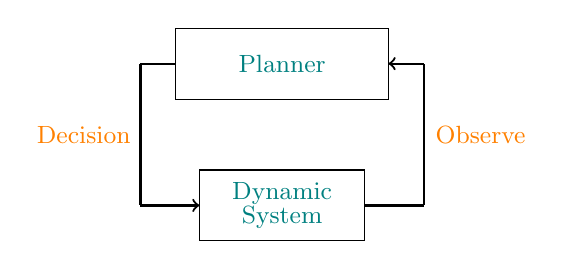
\begin{tikzpicture}[scale=0.6,font=\small,axis/.style={very thick, ->, >=sorangeth'}]

\draw [black=100](-2.25,-1.25) rectangle (2.25,0.25);
\node[teal] at(0,-0.5) {Planner};
%\node[black] at(0,-0.75) {};

\draw [black=100](-1.75,-4.25) rectangle (1.75,-2.75);
\node[teal] at(0,-3.25) {Dynamic};
\node[teal] at(0,-3.75) {System};

\node[orange] at(4.2,-2){\color{orange}{Observe}};


\node[orange] at(-4.2,-2){Decision};

\draw[thick,-](-2.25,-0.5)--(-3,-0.5);
\draw[thick,-](-3,-0.5)--(-3,-3.5);
\draw[thick,->](-3,-3.5)--(-1.75,-3.5);

\draw[thick,->](3,-0.5)--(2.25,-0.5);
\draw[thick,-](3,-3.5)--(3,-0.5);
\draw[thick,-](1.75,-3.5)--(3,-3.5);

\end{tikzpicture}
&
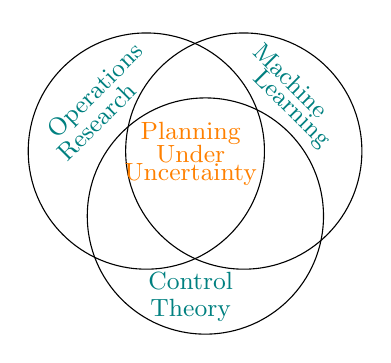
\begin{tikzpicture}[scale=0.75,font=\small,axis/.style={very thick, ->}]
\draw [] (0.9,0.5) circle (2);
\draw [] (-0.75,0.5) circle (2);
\draw [] (.25,-0.6) circle (2);
%\draw [] (-0.5,0.5) circle (2);
%\draw [] (0.5,-0.5) circle (2);
%\draw [] (-0.5,-0.5) circle (2);

\node[orange] at(0,0.8){Planning};

\node[orange] at(0,0.45){Under};
\node[orange] at(0,0.1){Uncertainty};

\node[teal,rotate=-45] at(1.7,1.7){Machine};
\node[teal,rotate=-45] at(1.7,1.2){Learning};

\node[teal,rotate=45] at(-1.6,1.5){Operations};
\node[teal,rotate=45] at(-1.6,1.0){Research};

\node[teal] at(-0,-1.7){Control};
\node[teal] at(-0,-2.2){Theory};
\end{tikzpicture}

\end{tabular}

\end{table}
%\caption*{No Explicit Labels; Control via Feedback }
\end{figure}

\end{frame}


\begin{comment}


\begin{frame}[fragile]{What? and What not?}

\begin{block}{What not?}
\begin{itemize}
\item Sequence $\neq$ Data Stream
\item Decisions are not right/wrong (no labels)
\end{itemize}
\end{block}

\begin{block}{What?}
\begin{itemize}
\item Stochastic Dynamical system
\item Decisions affects evolution
\end{itemize}

\end{block}
\begin{block}{Aim}
\centering Take {\color{orange}{control}} of the system
\end{block}
\end{frame}
\end{comment}

\begin{frame}[fragile]{Markov Decision Process (MDP)}
\begin{block}{MDP $\M=<\S,\A,P,g,\alpha>$}
\begin{itemize}
\item State space $\S=\{s^1,\ldots,s^n\}$
\item Action space $\A=\{a^1,\ldots,a^d\}$
\item Markovian Transition
\begin{align*}
Pr\{s_{t+1}=s'| s_t=s, a_t=a\}=p_a(s,s')
\end{align*}
\item Rewards $g_a(s)$ for action $a$ in state $s$
\item Policy: $u\colon \S\ra \A$ (induces a Markov chain with kernel $P_u$)
\item Value: $J_u(s)\eqdef \E\big[\sum_{t=0}^\infty \alpha^t g_{a_t}(s_t)|s_0=s,a_t=u(s_t)\big]$
\end{itemize}
\end{block}
\begin{block}{Aim for optimal}
Compute  $J^*(s)=\max_{u} J(s),\,\forall s\in \S$ and $u^*$ s.t $J_{u^*}=J^*$\footnote{$J^*\in \R{|\S|}$}
\end{block}
\begin{tikzpicture}[overlay]
\node[black] at (10,5) {\includegraphics[scale=0.25]{mouse-single.png}};
\end{tikzpicture}
\end{frame}


\begin{frame}[fragile]{Goal}
\begin{algorithm}[H]
%\caption*{Stochastic Multi-Arm Bandit}
\begin{algorithmic}[1]
\STATE{Input: $\M=<\S,\A,P,g,\alpha>$}
\STATE{solve_{MDP}(\M)\{}
\STATE{$\vdots$}
\STATE{\}}
\STATE{Output: $u^*$, $J^*$}
\end{algorithmic}

%\label{mab1}
\end{algorithm}

\end{frame}

\begin{frame}[fragile]{Different Paradigms in Decision Making}
\begin{block}{Classification}
\begin{itemize}
\item $(x,y)=(label,class)$, where $x\in \X$ and $y\in \Y=\{1,\ldots,K\}$
\item Assume we are given the densities $p(y|x),\,\forall y\in Y,\forall x\in \X$
\item Optimal decision is {\color{orange}{$h^*(x)=\arg\max_{y\in Y}p(y|x)$}}
\end{itemize}
\end{block}

\begin{block}{MDP}
\begin{itemize}
\item Assume we are given the model $M=<\S,\A,P,g,\alpha>$
\item Optimal decision is {\color{orange}{$u^*(s)=\arg\max_{a\in \A}(?)$}}
\end{itemize}
\end{block}

\begin{block}{News}
\centering
Overhead in computing $u^*$ ({\color{orange}{We are not lucky here}})
\end{block}

\end{frame}


\begin{frame}[fragile]{Challenge~I: {Curse-of-Dimensionality}}
\begin{block}{Complexity \cite{littman1995complexity}}
 $u^*$ can be computed in $poly(|\S|,|\A|)$
\end{block}

\begin{block}{Curse}
$|\S|$ grows exponentially in the number of state variables $s=(x_1,\ldots, x_q)$
\end{block}
\begin{block}{Example}
\begin{itemize}
\item A Queue has buffer size $n-1$, then $|\S|=n$
\item Queuing network has $p$ such queues, then $|\S|=n^q$
\item $n=10$, $q=5$, $|\S|=10^5$
\item Addition of an extra queue blows the state space $10$ times
\end{itemize}
\end{block}
$s=(x_1,\ldots, x_q)$, then $|\S|=|\X|^q$
\end{frame}

\begin{frame}[fragile]{Challenge~I: {Curse-of-Dimensionality}...}

\begin{itemize}
\item Huge State Space $\Rightarrow$  {\color{orange}{Exact Decision $u^*$ not possible}}
\item Compression by parameterization $\Rightarrow$ {\color{orange}{Approximate Decisions $\tilde{u}$}}
\end{itemize}

\begin{table}
\begin{tabular}{ccc}
\begin{minipage}{0.3\textwidth}
\begin{figure}
\includegraphics[scale=0.4]{mouse-single.png}
\caption*{Original}
\end{figure}
\end{minipage}
&
\begin{minipage}{0.3\textwidth}
\begin{figure}
\includegraphics[scale=0.4]{compress-mouse.png}
\caption*{How to compress???}
\end{figure}
\end{minipage}
&
\begin{minipage}{0.3\textwidth}
\begin{block}{Loss}
%{\color{orange}{Performance}}\\
{\color{orange}{How bad is $\tu$ in comparison to $u^*$?}}\\
\end{block}
\end{minipage}
\end{tabular}
\end{table}

\begin{block}{Keyword}
Approximate Dynamic Programming (ADP)
\end{block}
\end{frame}

\begin{frame}[fragile]{Challenge~II: {Lack of Model}}
\begin{itemize}
\item Model $P,g$ is not given
\item Noisy Sample Trajectories ({\color{orange}{$s_0-a_0-s_1-a_1-\cdots$}}), where ${\color{orange}{s_{t+1}\sim p_{a_t}(s_t,\cdot)}}$
\item Adaptive Online updates ({\color{orange}{$\theta(0), \theta(1), \ldots, \theta(t)$}})
\end{itemize}
\begin{table}
\begin{tabular}{cc}
\begin{minipage}{0.5\textwidth}
\begin{figure}
\includegraphics[scale=0.4]{traj.png}
\end{figure}
\end{minipage}
&
\begin{minipage}{0.5\textwidth}
\begin{block}{Question}
{\color{orange}{Stability?}}\\
{\color{orange}{$\theta(t)\ra \theta^*$ ?}}
\end{block}
\end{minipage}
\end{tabular}
\end{table}
\begin{block}{Keyword}
Reinforcement Learning; Stochastic Approximation
\end{block}

\end{frame}

\begin{frame}[fragile]{Research Contributions}
\textbf{\color{orange}{Developed ADP methods with provable performance guarantees}}
\begin{block}{Highlights}
\begin{itemize}
\item Novel basis in Tropical $(\min,+)$ algebra
\item Novel Monotone projection, Contraction Maps
\item Geometric conditions in linear optimization
\end{itemize}
\end{block}

\begin{block}{Publications}
Chandrashekar, L.; Bhatnagar, S., ``Approximate Dynamic Programming with $(\min,+)$ linear function approximation for Markov Decision Processes," $53^{rd}$ IEEE CDC, 2014\\
Chandrashekar, L.; Bhatnagar, S., ``A Generalized Reduced Linear Program for Markov Decision Processes," $29^{th}$ AAAI conference, 2015
\end{block}

\end{frame}
\begin{frame}[fragile]{Research Contributions}
\textbf{\color{orange}{Provided conditions that imply stability of multi-timescale stochastic approximation algorithms}}
\begin{block}{Highlights}
\begin{itemize}
\item Ordinary Differential Equation based analysis of Borkar et al
\item Umbrella result for various Reinforcement Learning algorithms
\end{itemize}
\end{block}

\begin{block}{Publication}
Chandrashekar, L. and  Bhatnagar, S. ``A Stability Criterion for Two Timescale Stochastic Approximation Schemes",  Automatica, 2017
\end{block}
\end{frame}
\begin{frame}[fragile]{Research Contributions}
\begin{block}{Crowd Sourcing}

Chandrashekar, L.;  Dubey, A.; Bhatnagar, S. and Chithralekha, B., ``A Markov Decision Process framework for predictable job completion times on crowdsourcing platforms", Proceedings of the Second {AAAI} Conference on Human Computation and Crowdsourcing, {HCOMP} 2014, Pittsburgh, Nov. 2-4, 2014
\end{block}
\begin{block}{Value Function}
Maity, R. K.; Chandrashekar, L.;  Padakandla, S.; Bhatnagar, S., `` Shaping Proto-Value Functions Using Rewards", European Conference on Artificial Intelligence 2016\\
\end{block}
\begin{block}{Constraint Sampling}
Chandrashekar, L.;  Bhatnagar, S and Szepesv\'{a}ri C., ``A Linearly Reduced Approximate Linear Program for Markov Decision Processes", submitted to IEEE Transactions on Automatic Control
\end{block}

\end{frame}



\section{Exact Dynamic Programming}

\begin{frame}[fragile]{Dynamic Programming}
\begin{block}{Values lead to Policy}
\begin{itemize}
\item$u^*(s)=\arg\max_{a\in \A}(?)$
\item $u^*(s)\eqdef \U(J^*)(s) =\arg\max_{a\in \A} (g_a(s)+\alpha p_a(s,\cdot)^\top J^*)$
\end{itemize}
\end{block}
\begin{block}{Greedy Principle}
{\color{orange}{Best = Current Best+ Future Best}}
\end{block}
\begin{block}{Bellman Equation}
\begin{align*}
J^*(s)&=\max_{a\in \A} g_a(s)+\alpha p_a(s,\cdot)^\top J^*\\
Q^*(s,a)&= g_a(s)+\alpha p_a(s,\cdot)^\top \max_{a\in \A} Q^*(\cdot,a)
\end{align*}
\end{block}

%\begin{block}{State-Action Values $Q^*\in \R^{|\S|\times |\A|}$}
%$u^*(s)\eqdef \U(Q^*)(s) =\arg\max_{a\in \A} Q^*(s,a)$
%\end{block}


%\begin{tikzpicture}[overlay]
%\node[black] at (10,7) {\includegraphics[scale=0.25]{mouse-single.png}};
%\end{tikzpicture}
\end{frame}


\begin{frame}[fragile]{Bellman Operator}
\begin{block}{Definition}
\begin{align*}
(TJ)(s)&\eqdef\max_{a\in \A} g_a(s)+\alpha p_a(s,\cdot)^\top J\\
%(HQ)(s,a)&\eqdef g_a(s)+\alpha p_a(s,\cdot)^\top \max_{a\in \A}Q(\cdot,a)
\end{align*}
\end{block}
\begin{block}{Properties of $T$}
\begin{itemize}
\item {Monotonicity:} $T J_1\geq T J_2, \mb \forall$ $J_1\geq J_2$
\item {Shift:} $T (J+k\one)= T J+\alpha k\one$
\item Monotonicity+Shift $\Rightarrow$ $T$ is contraction in $L_\infty$ norm
\end{itemize}
\end{block}
\begin{block}{Fixed Point Equation}
\centering $J^*=TJ^*$, %$Q^*=HQ^*$
\end{block}
\end{frame}


\begin{frame}[fragile]{Exact DP Algorithms}
\begin{block}{Value Iteration}
\begin{center}
Power Method: $J_{t+1}=T J_t$
\end{center}
\end{block}
\begin{block}{Policy Iteration}
\begin{center}
Evaluation: $J_{u_t}=T_{u_t} J_{u_t}$\\
Improvement: $u_{t+1}=\U J_{u_t}$
\end{center}
\end{block}

\begin{block}{Linear Programming}
\begin{align*}
J^*&=\arg\min_{J\in \R^{\S}} c^\top J\\
&\quad s.t. J\geq TJ
\end{align*}
\end{block}

\begin{center}
{\color{orange}{Convergent and Exact}}
\end{center}
\end{frame}


\begin{frame}[fragile]{Toy Grid World}

\begin{table}
\begin{tabular}{|c|c|c|}\hline
$\mb $&$\uparrow$	&$G$\\\hline
${\leftarrow}$	&$s$	&$\ra$\\\hline
$\mb$	&$\downarrow$	&$\mb$	\\\hline
\end{tabular}
\end{table}
\begin{itemize}
\item $S=X\times Y$, $A=\{\leftarrow,\rightarrow,\uparrow,\downarrow\}$, $\alpha=0.9$.
\item With $p=0.9$ move to desired position.
\item Reward at $G$ is $1$ otherwise $0$.
\end{itemize}

\begin{table}
\begin{tabular}{|c|c|c|}\hline
~$0$~	&~$0$~	&~$1$~\\\hline
$0$	&$0$	&$0$\\\hline
$0$ &$0$	&$0$\\\hline
\end{tabular}
\begin{tabular}{|c|c|c|}\hline
$0$	&$0.81$	&$1$\\\hline
$0$	&$0$	&$0.81$\\\hline
$0$ &$0$	&$0$\\\hline
\end{tabular}
\end{table}

\begin{table}
\begin{tabular}{|c|c|c|}\hline
$0.72$	&$1.53$	&$1.9$\\\hline
$0$	&$0.72$	&$1.53$\\\hline
$0$      &$0$	&$0.72$\\\hline
\end{tabular}
\begin{tabular}{|c|c|c|}\hline
$7.2$	&$8.1$	&$10$\\\hline
$6.56$	&$7.29$	&$8.1$\\\hline
$5.90$ &$6.56$	&$7.29$\\\hline
\end{tabular}
\end{table}
\begin{tikzpicture}[overlay]
\node[orange] at (4,4.25) {$TJ$};
\node[orange] at (6,4.25) {$T^2J$};

\node[orange] at (4,2.2) {$T^3J$};
\node[orange] at (6,2.2) {$J^*$};

\end{tikzpicture}
\end{frame}

\section{Approximate Dynamic Programming}


\begin{frame}[fragile]{Definitions}
\begin{block}{Norms}
Let $J_1,J_2\in \R^{|\S|}$
\begin{itemize}
\item $\norm{J_1-J_2}_{1,c}=\sum_{s\in \S} \left|J_1(s)-J_2(s)\right|$
\item $\norm{J_1-J_2}^2_{D}=\mfrac{1}{2}(J_1-J_2)^\top D \,(J_1-J_2)$, $D$ is a positive definite matrix
\item $\norm{J_1-J_2}_\infty=\max_{s\in \S}\left|J_1(s)-J_2(s)\right|$
\item $\norm{J_1-J_2}_{\infty,\psi}=\max_{s\in \S}\frac{\left|J_1(s)-J_2(s)\right|}{\psi(s)}$, for any $\psi>0 \in \R^{|\S|}$
\item $\norm{J_1-J_2}_{\infty}=\norm{J_1-J_2}_{\infty,\one}$ ($\one$ is vector all $1$)
\end{itemize}
\end{block}


\begin{block}{Superharomic Function}
For $f,g \in \R^{|\S|}$, $f$ is superharmonic to $g$ if $f\geq g$
\end{block}
\end{frame}

\begin{frame}[fragile]{Definitions}
\begin{block}{Maximal Inflation}
$\psi>0\in \R^{|\S|}$ then
\begin{align*}
\beta_\psi=\max_{a\in \A}\frac{\alpha p_a(s,\cdot)^\top \psi}{\psi(s)}
\end{align*}
\end{block}
\begin{block}{Lyapunov Function}
$\psi$ is a Lyapunov function if $\beta_\psi<1$
\end{block}

\begin{block}{Contraction Maps}
$M\colon \R^{|\S|}\ra\R^{|\S|}$
\begin{itemize}
\item {Monotonicity:} $M J_1\geq M J_2, \mb \forall$ $J_1\geq J_2$
\item {Shift:} $M (J+k\one)= M J+\gamma k\one$, $\gamma \in (0,1)$
\item Monotonicity+Shift $\Rightarrow$ $M$ is $\gamma$ contraction in $L_\infty$ norm
\end{itemize}
\end{block}

\end{frame}


\begin{frame}[fragile]{Approximate Dynamic Programming (ADP)}
\begin{block}{Why?}
Curse-of-Dimensionality (expensive to populate the table)
\end{block}
\begin{block}{What?}
{\color{orange}{ADP= Compression + DP}}
\end{block}
\begin{block}{How?}
Compute $\tj\approx J^*$ and $\tu=\U \tj$
\end{block}
\begin{block}{Promise of ADP [Dynamic Programming \& Optimal Control -Bertsekas]}
{\color{orange}{$\underbrace{||J_{\tilde{u}}-J^*||_\infty}_{\text{Performance Loss}} \leq \frac{2}{1-\alpha}\underbrace{||J^*-\tilde{J}||_\infty}_{\text{Prediction Error}}$}}
\end{block}
\end{frame}




\begin{frame}[fragile]{How to compress?}
\begin{block}{Regression Idea}
\begin{align*}
\tilde{J}&=\Phi \tr \\
&=\begin{bmatrix}\lvert& &\lvert  \\ \phi_1& \vdots& \phi_k\\ \lvert& & \lvert  \\ \end{bmatrix} \tr
\end{align*}
\end{block}
\begin{itemize}
\item $\Phi$ is a $|\S|\times k $ {\color{orange}{feature matrix}} and $\tr=(\tr(1),\ldots,\tr(k))\in \R^k$ is a weight vector.
\item Idea is to choose fewer basis i.e. $k<<|\S|$
\item $\Pi=\Phi (\Phi^\top D \Phi)^{-1}\Phi^\top D$ is the projection given by $\Pi J =\arg\min_{\Phi r}\norm{J-\Phi r}^2_D$
\end{itemize}

\end{frame}


\begin{frame}[fragile]{How to compute $\tj$?}

 Approximate Value Iteration{\color{orange}\ding{53}} $\Phi r_{t+1}= \Pi T (\Phi r_t)$ \,({\color{orange}{No fixed point}})

\begin{block}{Performance Guarantees}
\begin{itemize}
\item $\Pi T$ is not a contraction in $L_\infty$
\item Restricted conditions were given by \cite{melo2007q}:
$\norm{\phi_i}_\infty=1,\, \sum_i |\Phi(s,i)|\leq 1,\,\forall s\in \S, \,\forall i=1,\ldots,k$
\end{itemize}
\end{block}


{Approximate Policy Iteration}{\color{orange}\ding{53}}
\begin{align*}
&\Phi r_t=\Pi T_{u_t} \Phi J_{r_t} \\
&u_{t+1}=\U \Phi_{r_t}\,\text({\color{orange}{Poor~guarantee}})
\end{align*}

\begin{block}{Performance Guarantees}
\begin{itemize}
\item $\norm{\Phi r^*-J^*}_D\leq \frac{1}{1-\alpha}\norm{\Pi J^*-J^*}_D$ ({\color{orange}{Norm Mismatch}})
\item Leads to policy oscillations
\end{itemize}
\end{block}



\end{frame}

\begin{frame}[fragile]{How to Compress?}
\begin{block}{Approximate Linear Programming \cite{schweitzer1985generalized} {\color{orange}\ding{53}}}
\begin{align*}
 r^*&=\arg\min_{r\in \R^{k}} c^\top \Phi r\\
&\quad s.t. \Phi r\geq T \Phi r \,({\color{orange}{Large~Number~of~Constraints}})
\end{align*}
\end{block}
\begin{itemize}
\item Performance Guarantees - Studied by \cite{de2003linear}
\item {\color{orange}{What happens if we reduce constraints?}}
\end{itemize}
\end{frame}


\begin{frame}[fragile]{Research Goals}
\begin{table}
\begin{tabular}{ccc}

\begin{minipage}{0.3\textwidth}
\begin{figure}
\includegraphics[scale=0.2]{mouse-single.png}
\caption*{DP}
\end{figure}
\end{minipage}
&
\begin{minipage}{0.3\textwidth}
\begin{figure}
\includegraphics[scale=0.2]{compress-mouse.png}
\caption*{ADP}
\end{figure}
\end{minipage}
&
\begin{minipage}{0.3\textwidth}
%\begin{block}{???}
%{\color{orange}{Performance}}\\
{\color{orange}{$\norm{J^*-\tj}_\infty$?}}\\
%\end{block}
\end{minipage}
\end{tabular}
\end{table}
\begin{block}{Problems}
\begin{itemize}
\item Choose the right compression to eliminate norm mismatch?
\item Develop new tools to analyze constraint reduction?
\end{itemize}
\end{block}
\end{frame}
\begin{frame}[fragile]{Research Contributions}
\begin{block}{Novelty}
\begin{itemize}
\item Tropical linear function approximation
\item Projection onto sub-semimodules
\item Contraction maps and fixed points
\item Novel ideas mixing conventional and tropical linearity
\item Geometric conditions arising in linear programming
\end{itemize}
\end{block}
\begin{block}{Superharmonicity is key}
\end{block}
\end{frame}

\section{ADP in Tropical Algebra}

\begin{frame}[fragile]{Tropical Algebra}

\begin{block}{$\R_{\max}$ Semiring}
Addition: $x\op y\eqdef\max\{x,y\}$\\
Multiplication: $x\om y\eqdef x+y$
\end{block}


\begin{block}{$\R_{\min}$ Semiring}
Addition: $x\op y\eqdef\min\{x,y\}$,\\
Multiplication: $x\om y\eqdef x+y$
\end{block}

\begin{block}{Identity and Zero}
\begin{itemize}
\item $x\op \infty=x$
\item $x\om 0 =x$
\end{itemize}
\end{block}

\begin{block}{Semimodules}
$\R_{\max}^{|\S|}$, $\R_{\min}^{|\S|}$ are Semimodules
\end{block}
\end{frame}

\begin{frame}[fragile]{Applications}
\begin{block}{Synchronization}
$X_4=\max(X_1,X_2,X_3)$\\
Examples: Rail network, Shop floor
\end{block}


\begin{block}{Linearity}
\begin{itemize}
\item Consider a deterministic planning problem for a finite horizon $t$ with terminal cost $C(t)\colon \S\ra \R$
\item Let $\G\colon \S\ra \S$ be an operator that takes terminal cost $C(t)$ to first stage cost $C(0)$
\item $\G$ is $\minp$ linear, i.e.,
        \begin{itemize}
        \item $\G(C_1(t)\op C_2(t))=\G(C_1(t))\op \G(C_2(t))$
        \item $\G(\delta\om C(t))=\G(C(t))+\delta\one$
        \end{itemize}
\end{itemize}
\end{block}

\end{frame}


\begin{frame}[fragile]{Tropical Semiring}
\begin{block}{Literature}
\begin{itemize}
\item \cite{baccelli1994synchronization} - ``Synchronization and Linearity''
\item \cite{cohen1996kernels} - Projection onto Semimodules
\item \cite{akian2008max} - Deterministic Control
\item \cite{mceneaney2008curse,mceneaney2009convergence} - HJB PDEs
\item \cite{gaubert2011curse} - Pruning
\end{itemize}

\end{block}
\begin{block}{Our Work}
Chandrashekar Lakshminarayanan and Shalabh Bhatnagar, Approximate Dynamic Programming with $\minp$ linear basis for Markov Decision Processes, CDC 2014
\end{block}
\end{frame}



\begin{frame}[fragile]{Linear Span}

\begin{block}{Linear Basis in $\minp$ }
\begin{align*}
\tilde{J}&=\min\{\phi_{1}+\tr(1),\ldots,\phi_{k}+\tr(k)\}\subset \R_{\min}^{|\S|}\\
&=\Phi \om \tr \,\text{~is~a~sub-semimodule}
\end{align*}
\end{block}

\begin{block}{Exact Projection}
\begin{align*}
\Pi_M J&=\{\min \Phi \om r | \Phi \om r \geq J\},\,\text{minimum~is~component-wise}
\end{align*}
\begin{itemize}
\item Superharmonic: $\Pi_M J\geq J$
\item $k$ variables $|\S|$ inequalities
\end{itemize}
\end{block}

\end{frame}




\begin{frame}{Projections in the $(\min,+)$ basis}
\begin{itemize}
\item $f(x)=x^2$
\item $a=(a(j),j=1,\ldots,5)=(-0.8,-0.4,0,0.4,0.8)$
\item $\phi_j(x)=2|x-a(j)|$
\item $\tilde{f}(x)=\min\{\phi_1(x)+r(1),\ldots,\phi_5(x)+r(5)\}$
\end{itemize}
\begin{figure}\label{illust}
\begin{tikzpicture}[scale=0.6]
\begin{axis}[
xlabel=x,
ylabel=f(x),
ymin=0,
ymax=1.5
]
\only<1-> {\addplot[smooth,orange] plot file {mfile/f.dat}};
\only<2-2> {\addplot[dashed,teal] plot file {mfile/fo1.dat}};
\only<2-2> {\addplot[dashed,teal] plot file {mfile/fo2.dat}};
\only<2-2> {\addplot[dashed,teal] plot file {mfile/fo3.dat}};
\only<2-2> {\addplot[dashed,teal] plot file {mfile/fo4.dat}};
\only<2-2> {\addplot[dashed,teal] plot file {mfile/fo5.dat}};
\only<3-> {\addplot[dashed,teal] plot file {mfile/f1.dat}};
\only<3-> {\addplot[dashed,teal] plot file {mfile/f2.dat}};
\only<3-> {\addplot[dashed,teal] plot file {mfile/f3.dat}};
\only<3-> {\addplot[dashed,teal] plot file {mfile/f4.dat}};
\only<3-> {\addplot[dashed,teal] plot file {mfile/f5.dat}};
\only<4-> {\addplot[smooth,teal] plot file {mfile/fproj.dat}};
%   \addplot[dashed,black] plot file {mfile/f6.dat};
\end{axis}
\end{tikzpicture}
\caption{$(\min,+)$ LFA of $f(x)$}
\label{minptrans}
\end{figure}
\begin{block}{Superharmonic Property: $\tilde{f}\geq f$}
\end{block}
\end{frame}

\begin{frame}[fragile]{Use of Test Functions}
\begin{block}{Weak Projection}
\begin{align*}
\Pi^W_M J&=\{\min \Phi \om r | W\om \Phi \om r \geq W\om J\},\,W\text{~is~a~$m\times |\S|$test-matrix}
\end{align*}
\begin{itemize}
\item $W$ can be used to sample constraints
\item Let $s_1,\ldots,s_m$ be sampled states, then $W(i,s_i)=0,i=1,\ldots,m$ else $W(i,j)=\infty,\,\forall j\neq s_i$
\item $k$ variables $m$ constraints
\item Not superharomic; shows up as additional source of error
\end{itemize}
\end{block}
\end{frame}

\begin{frame}[fragile]{Composing $\Pi^W_M T$}
\begin{block}{Magic of $\minp$?}
{{$\Pi^W_M$ composes {\color{orange}{`nicely}'}with $T$}}
\end{block}
\begin{block}{Properties of $\Pi^W_M$}
\begin{itemize}
\item Fits well with $T$
    \begin{align*}
    TJ(s)&=\max \cdot\\
    TJ(s)&\geq \cdot\\
    &\geq \vdots\\
    &\geq \cdot
    \end{align*}
\item {Monotonicity:} $\Pi^W_M J_1\geq \Pi^W_M J_2, \mb \forall$ $J_1\geq J_2$
\item {Shift:} $\Pi^W_M J_1= \Pi^W_M J_2+\mathbf{1}$ for $J_1\eqdef J_2+\mathbf{1}$
\item $\Pi^W_M T$ is a contraction map in $L_\infty$
\end{itemize}
\end{block}

\end{frame}

\begin{frame}[fragile]{ADP in $\minp$}
\begin{block}{Approximate Value Iteration}
$\Phi \om r_{t+1}=\Pi^W_M T \Phi \om r_t$
\end{block}

\begin{block}{Main Theorem}
Let $\tilde{J}=\Phi \om \tr$ and $r^*\eqdef\arg\min_{r}\norm{J^*-\Phi \om r}_\infty$
%\begin{align*}
%||J^*-\tilde{J}||_\infty&\leq \frac{2}{1-\alpha}\arg\min_r||J^*-\Phi\om r||_\infty
%\end{align*}
%\begin{align*}
%||Q^*-\Phi\om \tr||_\infty\leq \frac{2}{1-\alpha}(||Q^*-\Phi\om r^*||_\infty+||\Phi\om r^*-\Pi_M^W \Phi\om r^*||_\infty).
%\end{align*}
\begin{align*}
\norm{J^*-\Phi\om \tr}_\infty\leq \frac{2}{1-\alpha}(\norm{J*-\Phi\om r^*}_\infty+\norm{\Phi\om r^*-\Pi_M^W \Phi\om r^*}_\infty).
\end{align*}
\begin{itemize}
\item Bound in the $L_\infty$ norm
\item Guaranteed Convergence $r_t \ra \tr$
\item Curse of Dimensionality reduction ($k$ variables and $m$ inequalities)
\item Error has two parts $i)$ approximation error $ii)$ weak projection error
\end{itemize}
\end{block}
\end{frame}





\begin{frame}{Experimental Results}
\begin{block}{}
$\mbox{ }$
$\mbox{ }$$\mbox{ }$
\includegraphics[scale=0.29]{mcar.png}
$\mbox{ }$
\includegraphics[scale=0.21]{actval.jpeg}\\
$\mbox{ }$\\
$\mbox{ }$
\includegraphics[scale=0.21]{basisval.jpeg}
$\mbox{ }$
\includegraphics[scale=0.19]{appval.jpeg}
\end{block}
\begin{tikzpicture}[overlay]
\node[orange] at (2,8.5) {Mountain Car};
\node[orange] at (8,8.5) {Exact Value};

\node[orange] at (2,4.5) {Basis};
\node[orange] at (8,4.5) {Approximate Value};
\end{tikzpicture}
\end{frame}


\begin{frame}[fragile]{Research Goals}
\begin{table}
\begin{tabular}{ccc}

\begin{minipage}{0.3\textwidth}
\begin{figure}
\includegraphics[scale=0.2]{mouse-single.png}
\caption*{DP}
\end{figure}
\end{minipage}
&
\begin{minipage}{0.3\textwidth}
\begin{figure}
\includegraphics[scale=0.2]{compress-mouse.png}
\caption*{ADP}
\end{figure}
\end{minipage}
&
\begin{minipage}{0.3\textwidth}
%\begin{block}{???}
%{\color{orange}{Performance}}\\
{\color{orange}{$\norm{J^*-J_{\tu}}$}}\\
%\end{block}
\end{minipage}
\end{tabular}
\end{table}
\begin{block}{Problems}
\begin{itemize}
\item Qs: Choose the right compression to eliminate norm mismatch?\\
{Ans:\color{teal}{$\minp$ linear basis}}+ \cite{melo2007q}
\item Develop new tools to analyze constraint reduction in LP?
\end{itemize}
\end{block}
\end{frame}

\section{Approximate Linear Programming (Recent Results)}

\begin{frame}[fragile]{Approximate Linear Programming}
\begin{block}{Literature}
\begin{itemize}
\item \cite{schweitzer1985generalized}
\item \cite{de2003linear}
\item \cite{de2004constraint}
\item \cite{desai2009smoothed}
\item \cite{petrik2010feature}
\end{itemize}
\end{block}

\begin{block}{Our Work}
Chandrashekar, L.; Bhatnagar, S., ``A Generalized Reduced Linear Program for Markov Decision Processes," AAAI, 2015\\
Chandrashekar, L.; Bhatnagar, S.; Szepesvari, C., ``A Linearly Relaxed Approximate Linear Program for Markov Decision Processes," submitted to IEEE Transactions on Automatic Control
\end{block}
\end{frame}
\begin{frame}[fragile]{Linear Programming}
\begin{block}{LP \cite{BertB}}
\begin{align*}
\min_{J\in \R^|\S|} &c^\top J\\
\text{s.t}\mb &J\geq T J
\end{align*}
\end{block}
\input{cartoonlp}
\begin{itemize}
\item LP is in $|\S|$ variables $|\S||\A|$ constraints
\item $c\geq 0 \in \R^{|\S|}$ is a non-negative vector
\item Searches in the bag of {\color{orange}{superharmonic}} functions $J\geq TJ\geq T^2J\geq J^*$
\item Complexity is $poly(|\S|,|\A|)$
\end{itemize}
\end{frame}

\begin{frame}[fragile]{Approximate Linear Programming (ALP)}
\begin{block}{ALP \cite{schweitzer1985generalized,de2003linear}}
\begin{align*}
\min_{r\in \R^k} &c^\top \Phi r\\
\text{s.t}\mb &\Phi r\geq T \Phi r
\end{align*}
\end{block}
\input{cartoonalp}
\begin{itemize}
\item ALP has $k$ variables $|\S||\A|$ constraints
\item {\color{orange}{superharmonic}} functions {\color{orange}{restricted}} to span of $\Phi$
\item ALP is feasible if $\one \in span(\Phi)$
\item $\underbrace{\norm{J^*-\tj}_{1,c}}_{\text{Error in ALP}}\leq \frac{2}{1-\alpha}\underset{r\in \R^k}{\min}\underbrace{||J^*-\Phi r||_{\infty}}_{\text{Best in the basis}}$
\end{itemize}
\end{frame}

\begin{frame}[fragile]{Saliency of ALP}
\begin{block}{}
$\underbrace{\norm{J^*-\tj}_{1,c}}_{\text{Error in ALP}}\leq \frac{2}{1-\alpha}\underset{r\in \R^k}{\min}\underbrace{||J^*-\Phi r||_{\infty}}_{\text{Best in the basis}}$
\end{block}
\begin{itemize}
\item $\norm{J^*-\tj}_{1,c}$, can choose $c$ to control the error
\item $\underbrace{\norm{J^*-\tj}_{1,c}}_{\text{Error in ALP}}\leq \frac{2}{1-\beta_\psi}\underset{r\in \R^k}{\min}\underbrace{||J^*-\Phi r||_{\infty,\psi}}_{\text{Best in the basis}}$
\item \cite{de2003linear,de2004constraint} choose $\psi$ to be large in un-important parts of state space
\end{itemize}
\begin{block}{Queuing Example}

\end{block}

\end{frame}

\begin{frame}[fragile]{Proofs}
\begin{block}{Feasibility}
$\min\{ c^\top \Phi r | \Phi r\geq T \Phi r, r\in \R^k\}$
\end{block}
\cite{de2003linear} show that ALP is feasible if $\one$ is in the span of $\Phi$.
\begin{block}{Proof}
Let $\epsilon=\min_r \norm{J^*-\Phi r}_\infty=\norm{J^*-\Phi r^*}_\infty$
\begin{align*}
\norm{J^*-T (\Phi r^*)}_\infty=\alpha \epsilon\,\quad(\text{Contraction~of~}\,T)\\
\Phi r^* \geq T \Phi r^* -(1+\alpha)\epsilon\,\quad(\text{translate~along~}\,\one)\\
\Phi r^* + k\one\geq T \Phi r^* -(1+\alpha)\epsilon +\alpha k\one\,\quad(\text{pick}\,k=\frac{1+\alpha}{1-\alpha})\\
\end{align*}
\end{block}
\end{frame}

\begin{frame}[fragile]{Reduced Linear Program}
\begin{block}{RLP \cite{de2004constraint}}
\begin{align*}
\min_{r\in \N\subset\R^k} &c^\top \Phi r\\
\text{s.t}\mb &\Phi r (s)\geq g_a(s)+\alpha p_a(s,\cdot)^\top \Phi r,\,\forall s\in \I
\end{align*}
\input{cartoonrlp}
\begin{itemize}
\item $\N$ is chosen to ensure boundedness
\item $\I$ is an index set of cardinality $m$ containing state-action pairs
\item Not superharmonic (can be handled)
\end{itemize}
\end{block}
\end{frame}
\begin{frame}[fragile]{RLP: Details}
\begin{block}{\cite{de2004constraint}}
Under suitable conditions, for a small $\epsilon>0$
\begin{align*}
\norm{J^*-\hj}_{1,c}\leq \norm{J^*-\tj}_{1,c}+\epsilon\norm{J^*}_{1,c}
\end{align*}
\end{block}
\begin{itemize}
\item $\N$ contains $\tr$ (solution to ALP)
\item Let $\mu^*=(1-\alpha)c^\top (I-\alpha P_{u^*})^{-1}$
\item For a Lyapunov function $\psi$, define $\mu^*_{\psi}(s,a)=\frac{\mu^*(s)\psi(s)}{|\A|{\mu^*}^\top \psi}$
\item Let $\theta=\frac{1+\beta_{\psi}}{2}\frac{{\mu^*}^\top \psi}{c^\top J^*}\sup_{r\in \N}\norm{J^*-\Phi r}_{\infty,\psi}$
\item Result holds with probability $1-\delta$ for RLP with $m$ constraints sampled from $\mu^*_{\psi}$, when $m\geq \frac{16|\A|\theta}{(1-\alpha)\epsilon}\big(k\ln \frac{48|\A|\theta}{(1-\alpha)\epsilon}+\ln\frac{2}{\delta}\big)$
\end{itemize}
\end{frame}
\begin{frame}[fragile]{Constraint Reduction- Gap in Theory}
\begin{block}{\cite{de2004constraint}}
\begin{itemize}
\item No apriori way to choose $\N$
\item For unbounded $\N$ the result is vacuous
\item Sampling distribution depends on $u^*$
\item Use of other sampling distribution will have importance sampling ratio
\item Depends on combinatorial arguments (VC-dimension)
\item Empirical results good for variety of sampling distribution (no knowledge of $u^*$) on various domains (Tetris, Queues etc)
\end{itemize}
\end{block}
\begin{block}{Gap}
Theory does not explain empirical evidence
\end{block}
\end{frame}

\begin{frame}[fragile]{Linearly Relaxed Approximate Linear Program}
\begin{block}{LRALP}
\begin{align*}
&{\min}_r \,\mb c^\top \Phi r\,,\\
&\text{s.t.} \,\,\, W^\top  \Phi r\geq W^\top T \Phi r\,\\
\end{align*}
\end{block}
\begin{itemize}
\item $W$ is a $m\times |\S||\A|$ matrix with non-negative entries
\item LRALP is has $k$ variables $m$ constraints
\item $W$ can encode sampling as well as linear projection of constraints
\end{itemize}
\end{frame}

\begin{frame}[fragile]{Novel Contraction Operators}

\begin{block}{Superharmonic Property}
ALP as well as $\minp$ algebra
\end{block}
\begin{block}{Least Upper Bound $\Gamma$}
\begin{align*}
\begin{split}
&r_c\eqdef\arg\min_{r} \,\, c^\top \Phi r\,,\\
&\text{s.t.} \mb \Phi r\geq  TJ\,,\\
&(\Gamma J)(s)\eqdef(\Phi r_{e_s,J})(s),\quad s=1,\ldots,|\S|\,.
\end{split}
\end{align*}
\end{block}

\begin{block}{Approximate Least Upper Bound $\hg$}
\begin{align*}
&\hat{r}_c={\arg\min}_{r} \,\mb c^\top \Phi r\,,\\
&\text{s.t.} \,\,\, W^\top  \Phi r\geq W^\top TJ\,\\
&(\hg J)(s)\eqdef(\Phi \hr_{e_s,J})(s),\, s=1,\ldots,|\S|\,.
\end{align*}
\end{block}
\end{frame}


\begin{frame}[fragile]{Main Result - Prediction Error}
\begin{align*}
\norm{J^*-\hj}_{1,c}\leq \frac{2}{1-\alpha}( 3\norm{J^*-\Phi r^*}_{\infty}+ \norm{\Gamma J^*-\hg J^*}_{\infty})
\end{align*}
\begin{itemize}
\item Error has two parts $i)$ Approximation Error $ii)$ Projection Error
\item The bound is deterministic
\item Factor $3$ is a proof artifact
\item Does not depend on sampling
\item Can be stated in $\norm{\cdot}_{\infty,\psi}$
\end{itemize}
\end{frame}

\begin{frame}[fragile]{Main Result - Constraint Sampling}
\begin{block}{Conic Conditions}
Let $\S_0\subset \S$ such that the rows of $\Phi$ lies in the conic span of $\Phi(\S_0,\cdot)$ with co-efficient matrix $\Lambda$. Then
\begin{align*}
\norm{ \Gamma J^*-\hg J^* }_{\infty,\psi}\leq (3+\norm{\Lambda \psi}_{\infty,\psi})\inf_r\norm{J^*-\Phi r}_{
\infty,\psi}
\end{align*}
\end{block}
\begin{itemize}
\item Geometric condition for linear programs
\item Can ensure for variety of linear approximation such as tile coding, state aggregators, separable bases
\item $|\S_0|$ is purely geometric requirement, unlike $m$ samples for RLP
\end{itemize}
\end{frame}


\begin{frame}[fragile]{Properties of new operators}
\begin{itemize}
\item Define $\F_J\eqdef\{\Phi r | \Phi r\geq TJ \}$
\item $\F_J$ contains all functions superharmonic with $TJ$
\item {Monotonicity:} $\Gamma J_1\geq \Gamma J_2, \mb \forall$ $J_1\geq J_2$
\item {Shift:} $\Gamma (J_1+k\one)= \Gamma J_1+ k\one$
\item $\Gamma$ and $\hg$ are $L_{\infty,\psi}$ contraction maps
\end{itemize}
\input{schematic}
\end{frame}


\begin{frame}[fragile]{Experimental Results}
Queue with $10^4$ states.
\begin{table}
\begin{tabular}{|c|c|c|c|c|}\hline
Error Term&     $W_i$&  $W_c$& $W_a$& $W_r$ \\\hline
$\et$ & $39$    &$84$& $54.15$& $251.83$ \\\hline
\end{tabular}
\end{table}

\begin{table}
\begin{center}
%\resizebox{\columnwidth}{!}{
\begin{tabular}{|c|c|c|c|c|}\hline
Error Terms&    $W_i$&  $W_c$& $W_a$& $W_r$ \\\hline
$||J^*-\hj||_{1,c}$ for $\zeta=0.9$& $32$&      $32$& $220$& $5.04\times 10^4$ \\\hline
$||J^*-\hj||_{1,c}$ for $\zeta=0.999$& $110$&   $180.5608$& $82$& $1.25\times 10^7$ \\\hline
\end{tabular}
\end{center}
%}
\caption*{Prediction Errors.}
\label{perf1}
\end{table}
\begin{block}{Matrices}
$W_a$- Aggregation, $W_i$ -Ideal Sampler, $W_c$ - Sample using $c$, $W_r$ - Random.
\end{block}
\end{frame}

\section{Future Plans}
\begin{frame}[fragile]{Future Research Goals}
\begin{itemize}
\item Large scale MDPs based on the LP
\item Finite time behaviour of Reinforcement Learning (RL) algorithms
\item Regret minimization for RL
\item Deep Reinforcement leanring
\end{itemize}
\end{frame}
\begin{frame}[fragile]{Teaching Plan}
\textbf{Computer Science}
\begin{enumerate}
\item Introduction to Programming
\item Design and Analysis of Algorithms
\item Discrete mathematics for Computer Science
\item Linear algebra
\item Programming and Data Structure
\item Probability, Stochastic Process and Statistics
\item Engineering Mathematics
\end{enumerate}
\textbf{Electrical Engineering}
\begin{enumerate}
\item Digital Design
\item Microprocessors
\item Network/Circuit Theory
\item Analog Electronics
\item Linear Integrated Circuits
\item Signals and Systems
\item Classical and Modern Control Theory
\end{enumerate}
\end{frame}
\begin{frame}[fragile]{Advanced Courses}
\begin{itemize}
\item Reinforcement Learning
\item Stochastic Approximation Algorithms
\item Optimization
\end{itemize}
\end{frame}

\begin{frame}[fragile]{Acknowledgements}
\begin{itemize}
\item Shalabh Bhatnagar
\item Csaba Szepesvari
\item Srujana Sadula
\item Ayush Dubey
\item Rishabh Singla
\item Sindhu Padakandla
\item Rajkumar Maity
\item Chithralekha Balamurugan
\item Sujit Gujar
\end{itemize}
\end{frame}

\begin{frame}[allowframebreaks]{References}
\bibliographystyle{plainnat}
\bibliography{ref}
\end{frame}

\end{document}
